\documentclass[tikz,border=10pt]{standalone}
\usepackage{amsmath}
\definecolor{bg}{HTML}{171D2B}
\definecolor{acc}{HTML}{F7B538}
\definecolor{line}{HTML}{8FA3C8}
\pagecolor{bg}
\color{white}
\begin{document}
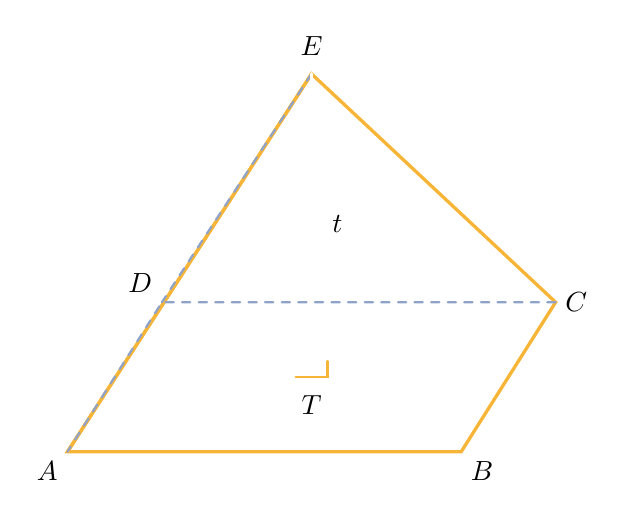
\begin{tikzpicture}[scale=1.0,line cap=round]
  % titik-titik alas (segiempat dalam proyeksi)
  \coordinate (A) at (0,0);
  \coordinate (B) at (5,0);
  \coordinate (C) at (6.2,1.9);
  \coordinate (D) at (1.2,1.9);
  % puncak limas
  \coordinate (E) at (3.1,4.8);
  % titik proyeksi puncak ke alas = pusat alas
  \coordinate (T) at (3.1,0.95);
  % titik tengah AB untuk menandai rusuk alas
  \coordinate (M) at (2.5,0);
  % sisi yang terlihat (tebal, aksen)
  \draw[acc,very thick] (A) -- (B) -- (C) -- (E) -- cycle;
  \draw[acc,very thick] (E) -- (A);
  % sisi tersembunyi (putus-putus)
  \draw[line,dashed,thick] (C) -- (D) -- (A);
  \draw[line,dashed,thick] (E) -- (D);
  % tinggi limas: tegak lurus alas, dari puncak ke titik proyeksi T
  \draw[white,very thick] (E) -- (T);
  \draw[acc,line width=1pt] (2.9,0.95) -- (3.3,0.95) -- (3.3,1.15); % tanda siku di T
  % label titik sudut
  \node[below left]  at (A) {$A$};
  \node[below right] at (B) {$B$};
  \node[right]       at (C) {$C$};
  \node[above left]  at (D) {$D$};
  \node[above=3pt]   at (E) {$E$};
  \node[below=3pt]   at (T) {$T$};
  \node[right=4pt]   at (3.1,2.9) {$t$};
\end{tikzpicture}
\end{document}
